% !TEX root = ../tesi.tex

\section{Context}

Network security is a critical concern for virtually every organization, from small businesses to large enterprises and public institutions. All of them rely on computer networks to support their operations, and all of them are exposed to the risk of unauthorized access, data breaches, and service disruptions. As a result, enforcing a well-defined and correct security policy is not optional, but instead is a fundamental operational requirement.

Modern enterprise networks are characterized by growing complexity: hundreds of interconnected nodes, heterogeneous services, and security policies that must be consistently enforced across distributed infrastructure. Moreover, network topologies are not static: new services are deployed, nodes are added or removed, and connectivity requirements evolve continuously, making security management an ongoing and demanding task. The cost of managing network security in this context is significant, as it requires specialized expertise, advanced planning, and constant monitoring~\cite{automation-survey}.

A central challenge in this landscape stems from the evolution of network security architectures. Traditionally, a single perimeter firewall was sufficient to protect a network by controlling traffic at its boundary. However, as networks grew in scale and complexity, this model proved inadequate: a single point of control cannot enforce fine-grained policies across a heterogeneous internal topology. Modern networks have therefore evolved toward microsegmentation, deploying multiple packet-filtering firewall instances strategically distributed across the topology to enforce security policies at a much more granular level~\cite{novel-abstraction}. This distributed approach offers clear advantages such as enabling finer-grained traffic control, reduces single points of failure, and allows security policies to be enforced closer to the traffic sources, but it also introduces considerable management complexity. Each firewall instance must be individually configured with a set of filtering rules, and those rules must collectively enforce the intended security policy across the entire network, without conflicts or gaps.

In this context, the configuration of firewalls becomes a critical task. On one hand, overly permissive rules may allow unauthorized traffic to reach sensitive resources, exposing the network to attacks. On the other hand, overly restrictive rules may block legitimate traffic, degrading service availability and causing operational disruptions. Both failure modes carry significant consequences, and yet both are common outcomes of manual configuration process which is inherently prone to errors especially for large-scale networks~\cite{atomizing}.

The gap between the complexity of modern networks and the limitations of manual security management calls for automated approaches that can generate correct and optimal firewall configurations without human intervention. It is in this context that VEREFOO was developed: a tool for the automated, formally correct allocation and configuration of distributed firewalls, designed to bridge exactly this gap.

% todo: Rifare gli schemi di:
% - perimetral firewall architecture
% - distributed firewall architecture

\begin{figure}[htbp]
    \centering
    \begin{minipage}[t]{0.48\textwidth}
        \centering
        \includegraphics[width=\textwidth]{images/Perimetral-FW.jpg}
        \subcaption{Traditional perimeter firewall architecture.}
        \label{fig:perimetral-fw}
    \end{minipage}
    \hfill
    \begin{minipage}[t]{0.48\textwidth}
        \centering
        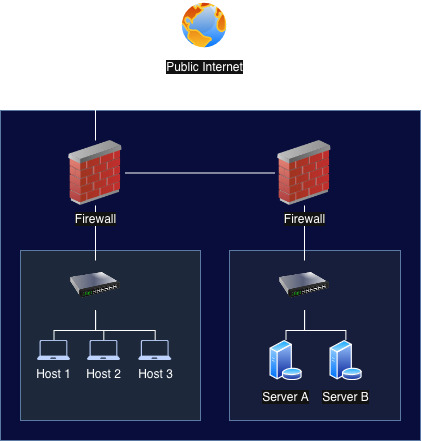
\includegraphics[width=\textwidth]{images/Distributed-FW-white.jpg}
        \subcaption{Distributed firewall architecture (microsegmentation).}
        \label{fig:distributed-fw}
    \end{minipage}
    \caption{Evolution of network security architectures: from a single perimeter firewall to distributed packet-filtering instances deployed across the topology.}
    \label{fig:fw-architectures}
\end{figure}

\section{VEREFOO}

\subsection{Overview}

% - Verefoo serve per automatizzare l'allocazione e la configurazione dei firewall di tipo packet-filtering in una rete
% - Il grande vantaggio è che l'allocazione e la configurazione dei firewall avviene in maniera automatica, senza intervento umano
% - Input: topologia di rete + insieme di NSR (Network Security Requirements)
% - Output: allocazione ottimale dei firewall nella rete + configurazione delle regole
% - Garanzie: correttezza formale e ottimalità globale
% - Approccio: encoding come problema MaxSMT, risolto con Z3
% - Obiettivo di ottimizzazione: minimizzare numero di firewall e regole allocate
% - Input: Service Graph + NSR 
% - Output: Firewall Allocation Schema (FAS) 
% - Verefoo é stato testato su reti reali e sintetiche (Stanford e CESNET) dimostrando affidabilitá e scalabilitá
% - Limite: approccio monolitico  $\rightarrow$  non scala al crescere della rete o degli NSR

VEREFOO (VErification REasoning on Firewall Optimization) is a tool designed to automate the allocation and configuration of packet-filtering firewalls in a network, eliminating the need for manual intervention entirely~\cite{verefoo}. Given a network topology and a set of Network Security Requirements (NSRs) --- high-level specifications describing which traffic flows must be allowed or denied between network endpoints~\cite{twofold} --- VEREFOO automatically determines where firewalls should be placed within the topology and generates the corresponding filtering rules for each allocated instance. The resulting configuration is expressed in a vendor-independent format, which can then be translated into concrete rules for specific implementations such as iptables, BPF, or OVS.

% todo: add a figure illustrating the input and output of VEREFOO, showing a network topology with NSRs as input and the resulting firewall allocation and rule sets as output

The tool provides three formal guarantees. \textit{Automation} ensures that no human intervention is required at any stage of the process. \textit{Formal correctness} guarantees that the generated configuration satisfies all specified NSRs by construction, eliminating the risk of undetected misconfigurations. \textit{Optimality} ensures that both the number of allocated firewall instances and the number of generated rules are minimised, reducing resource consumption and improving performance. These properties are achieved by encoding the firewall allocation and configuration problem as a partial weighted Maximum Satisfiability Modulo Theories (MaxSMT) instance, which is then solved using the Z3 SMT solver. The hard constraints of the problem encode the correctness requirements, while the soft constraints encode the optimality objectives; the solver finds a solution that satisfies all hard constraints and maximises the sum of satisfied soft constraint weights.


\subsection{Network Security Requirements}

Network Security Requirements (NSRs) are the high-level specification of the security policy that a network must enforce. Rather than describing firewall rules directly, NSRs express what the administrator intends: which traffic flows between pairs of endpoints must be permitted and which must be denied. This level of abstraction decouples the intent of the security policy from its low-level implementation, allowing VEREFOO to take full responsibility for translating requirements into concrete filtering rules~\cite{verefoo}.

Each NSR refers to a specific traffic flow, identified by five attributes: source address, destination address, transport protocol, source port, and destination port. The administrator specifies, for each such flow, whether it must be reachable (i.e., allowed end-to-end through the network) or isolated (i.e., blocked). VEREFOO supports four different policy modes that determine how the requirements are interpreted: \textit{whitelisting}, where all traffic is blocked by default and only explicitly allowed flows are permitted; \textit{blacklisting}, where all traffic is allowed by default and only explicitly listed flows are denied; and two mixed modes (\textit{rule-oriented specific} and \textit{security-oriented specific}), which accept both reachability and isolation requirements without a fixed default behavior, differing in how unspecified flows are handled~\cite{verefoo}.

NSRs are provided to VEREFOO as part of its input, alongside the network topology. Internally, they are represented and stored as a structured set of logical constraints, expressed in a vendor-independent intermediate language. A higher-level specification language is also supported, from which the corresponding medium-level NSRs are automatically derived through a translation step. VEREFOO processes this set together with the Allocation Graph derived from the topology, and encodes each NSR as a hard constraint in the MaxSMT problem: the solver is required to find a firewall allocation and rule set that satisfies all of them without exception. NSRs that are satisfied by the same firewall rules are grouped and handled jointly to minimise the total number of generated rules, while each unresolvable conflict or missing coverage results in a non-enforceability report to the administrator~\cite{verefoo,twofold}.

\subsection{Service Graph}

A Service Graph (SG) is the logical representation of a virtual network: a directed graph in which nodes represent Network Functions (NFs) such as web servers, load balancers, caches, or client subnetworks while edges represent the connectivity between them. The SG captures all possible end-to-end traffic paths through the network at an abstract level, without exposing low-level forwarding infrastructure such as switches and routers. It is defined taking into consideration solely the services that the network must provide, independently of any security consideration~\cite{verefoo}.

The SG serves as the structural input to VEREFOO: it defines the space of possible firewall positions and the traffic paths that any allocated firewall must be able to intercept. To make this explicit, VEREFOO automatically derives an internal representation called the \textit{Allocation Graph} (AG) from the SG. For each link between any pair of nodes in the SG, the AG introduces a placeholder element called an \textit{Allocation Place} (AP) which represents a candidate position where a firewall instance may be allocated. Those Allocation Places are then used by VEREFOO during the optimal placement of firewalls. Optionally, Verefoo allow to manually constrain this process by forcing a firewall into a specific AP or excluding certain APs from consideration, for example to model pre-existing hardware firewalls that cannot be moved~\cite{verefoo}.

VEREFOO uses the Allocation Graph (AG) jointly with the Network Security Requirements (NSRs) to formulate the MaxSMT problem. Each AP corresponds to boolean decision variable that the solver uses to determines the optimal firewall placement and what filtering rules each firewall should enforce, such that all NSRs are satisfied and the total number of allocated firewalls and rules is minimised.

% todo: add figures:
% - service graph without firewall


\subsection{VEREFOO Output}

When the MaxSMT problem is solved successfully, VEREFOO produces two complementary outputs~\cite{verefoo}. The first is the \textit{firewall allocation scheme}: an updated version of the Allocation Graph in which each selected Allocation Place hosts an active firewall instance, with the minimum number of firewalls necessary to enforce all NSRs. The second is the \textit{Filtering Policy} (FP) for each allocated firewall: a complete, auto-generated rule set that defines how the firewall must handle every traffic flow passing through it. Each FP is expressed in a vendor-independent abstract language, making it independent of any specific firewall implementation. It consists of a default action (either drop-all in whitelisting mode, or allow-all in blacklisting mode) and a minimal set of explicit rules covering the traffic flows specified by the NSRs. Both the default action and the explicit rules are guaranteed to be anomaly-free, with no conflicts or redundancies among them.

Together, these two outputs constitute the full security configuration of the network at the logical level of the Service Graph, independent of the physical infrastructure. A subsequent translation step converts the abstract filtering policies into concrete rules for specific implementations such as iptables, BPF, or OVS~\cite{verefoo}. If instead no solution exists, for example because user-defined constraints on the AG have excluded all viable firewall positions, VEREFOO returns a non-enforceability report in place of the configuration.

% todo: insert image: allocation graph, with allocation places
%?: Verefoo non ragiona su singoli pacchetti, ma su flussi di traffico %todo => spiegare benefici

\subsection{Verefoo validation}

VEREFOO has been validated on both synthetic and real-world network topologies, including well-known benchmarks such as the Stanford and CESNET networks, demonstrating reliability and scalability across a range of network sizes and requirement sets~\cite{verefoo}.

Despite these strengths, VEREFOO's monolithic approach has a fundamental scalability limitation: the entire set of NSRs and the full network topology are encoded into a single MaxSMT problem. As the number of requirements or the size of the network grows, the complexity of the problem increases significantly, leading to prohibitive computation times. This limitation motivates the development of more efficient alternatives, starting with React-VEREFOO.

% todo: add sentence like: "furhter details on the VEREFOO approach and its validation can be found in Chapter~\ref{chap:implementation_validation}." 

\section{React-VEREFOO}

In operational environments, network security policies are not static: NSRs evolve over time as new services are deployed, topology changes occur, or threat models are updated~\cite{autonomous}. A fundamental limitation of the monolithic approach used by VEREFOO is that any change to the NSR set triggers a full recomputation of the firewall configuration from scratch. React-VEREFOO addresses this by offering a more efficient approach in the dynamic context described above, avoiding the need to discard a valid existing configuration when only a small portion of the requirements has changed~\cite{reactverefoo}.

React-VEREFOO takes as input both the existing firewall configuration and the updated set of security requirements, and computes only the minimal changes needed to bring the network into compliance. Rather than reconsidering the entire problem, it identifies which requirements are new, which have been removed, and which remain unchanged. Only the newly added requirements drive the reconfiguration: the approach determines which parts of the network are affected and restricts the solver to those areas, leaving the rest of the configuration untouched. The result is an updated firewall allocation and rule set that satisfies all current requirements, with the same guarantees of correctness and optimality as VEREFOO.

Experimental results show that React-VEREFOO is significantly more efficient than vanilla VEREFOO when the proportion of modified NSRs is small, as the reduced problem size leads to much shorter solving times. However, when a large fraction of the requirements changes, the benefits is reduced and React-VEREFOO's performance becomes comparable to that of the monolithic approach. This observation motivates the approach investigated in this thesis: by pushing the incremental logic to its extreme - introducing only one new NSR per iteration - the proportion of modified requirements is always minimised, potentially achieving consistent speedups regardless of the total number of requirements.

% todo: add illustration of React-VEREFOO approach; showing the difference between VEREFOO Vanilla